%\documentclass[<options>]{elsarticle}
\documentclass [sort&compress] {elsarticle}
\usepackage{graphicx}% Include figure files

\bibliographystyle{elsarticle-num}
\begin{document}

\section*{Supplementary material}


\begin{figure}[!h]

\includegraphics[width=0.5\textwidth]{FigS1a}%

\includegraphics[width=0.5\textwidth]{FigS1b}
\caption{\label{figS1}
Ideality factor as a function of the iron concentration, temperature (a), and dopant (boron) concentration (b).
FI--SRH case.
$N_\mathrm{A}$ cm$^{-3}$: $10^{15}$ (surface 1), $10^{16}$ (2), $10^{17}$ (3).
$T$, K: 290 (4), 315 (5), 340 (6).
}%
\end{figure}


\begin{figure}[!h]

\includegraphics[width=0.5\textwidth]{FigS2a}%

\includegraphics[width=0.5\textwidth]{FigS2b}

\includegraphics[width=0.5\textwidth]{FigS2c}
\caption{\label{figS2}
Fermi level position as a function of the temperature and dopant (boron) concentration.
Data calculated by using SCAPS.
Base depth $x$, $\mu$m: 26 (a), 0.26 (b), 0.028 (c).
}%
\end{figure}


\begin{figure}

\includegraphics[width=0.5\textwidth]{FigS3a}%

\includegraphics[width=0.5\textwidth]{FigS3b}

\includegraphics[width=0.5\textwidth]{FigS3c}
\caption{\label{figS3}
The probability of hole occupation of $\mathrm{Fe}_i$ level as a function of the temperature and dopant (boron) concentration.
Base depth $x$, $\mu$m: 26 (a), 0.26 (b), 0.028 (c).
}%
\end{figure}


\begin{figure}
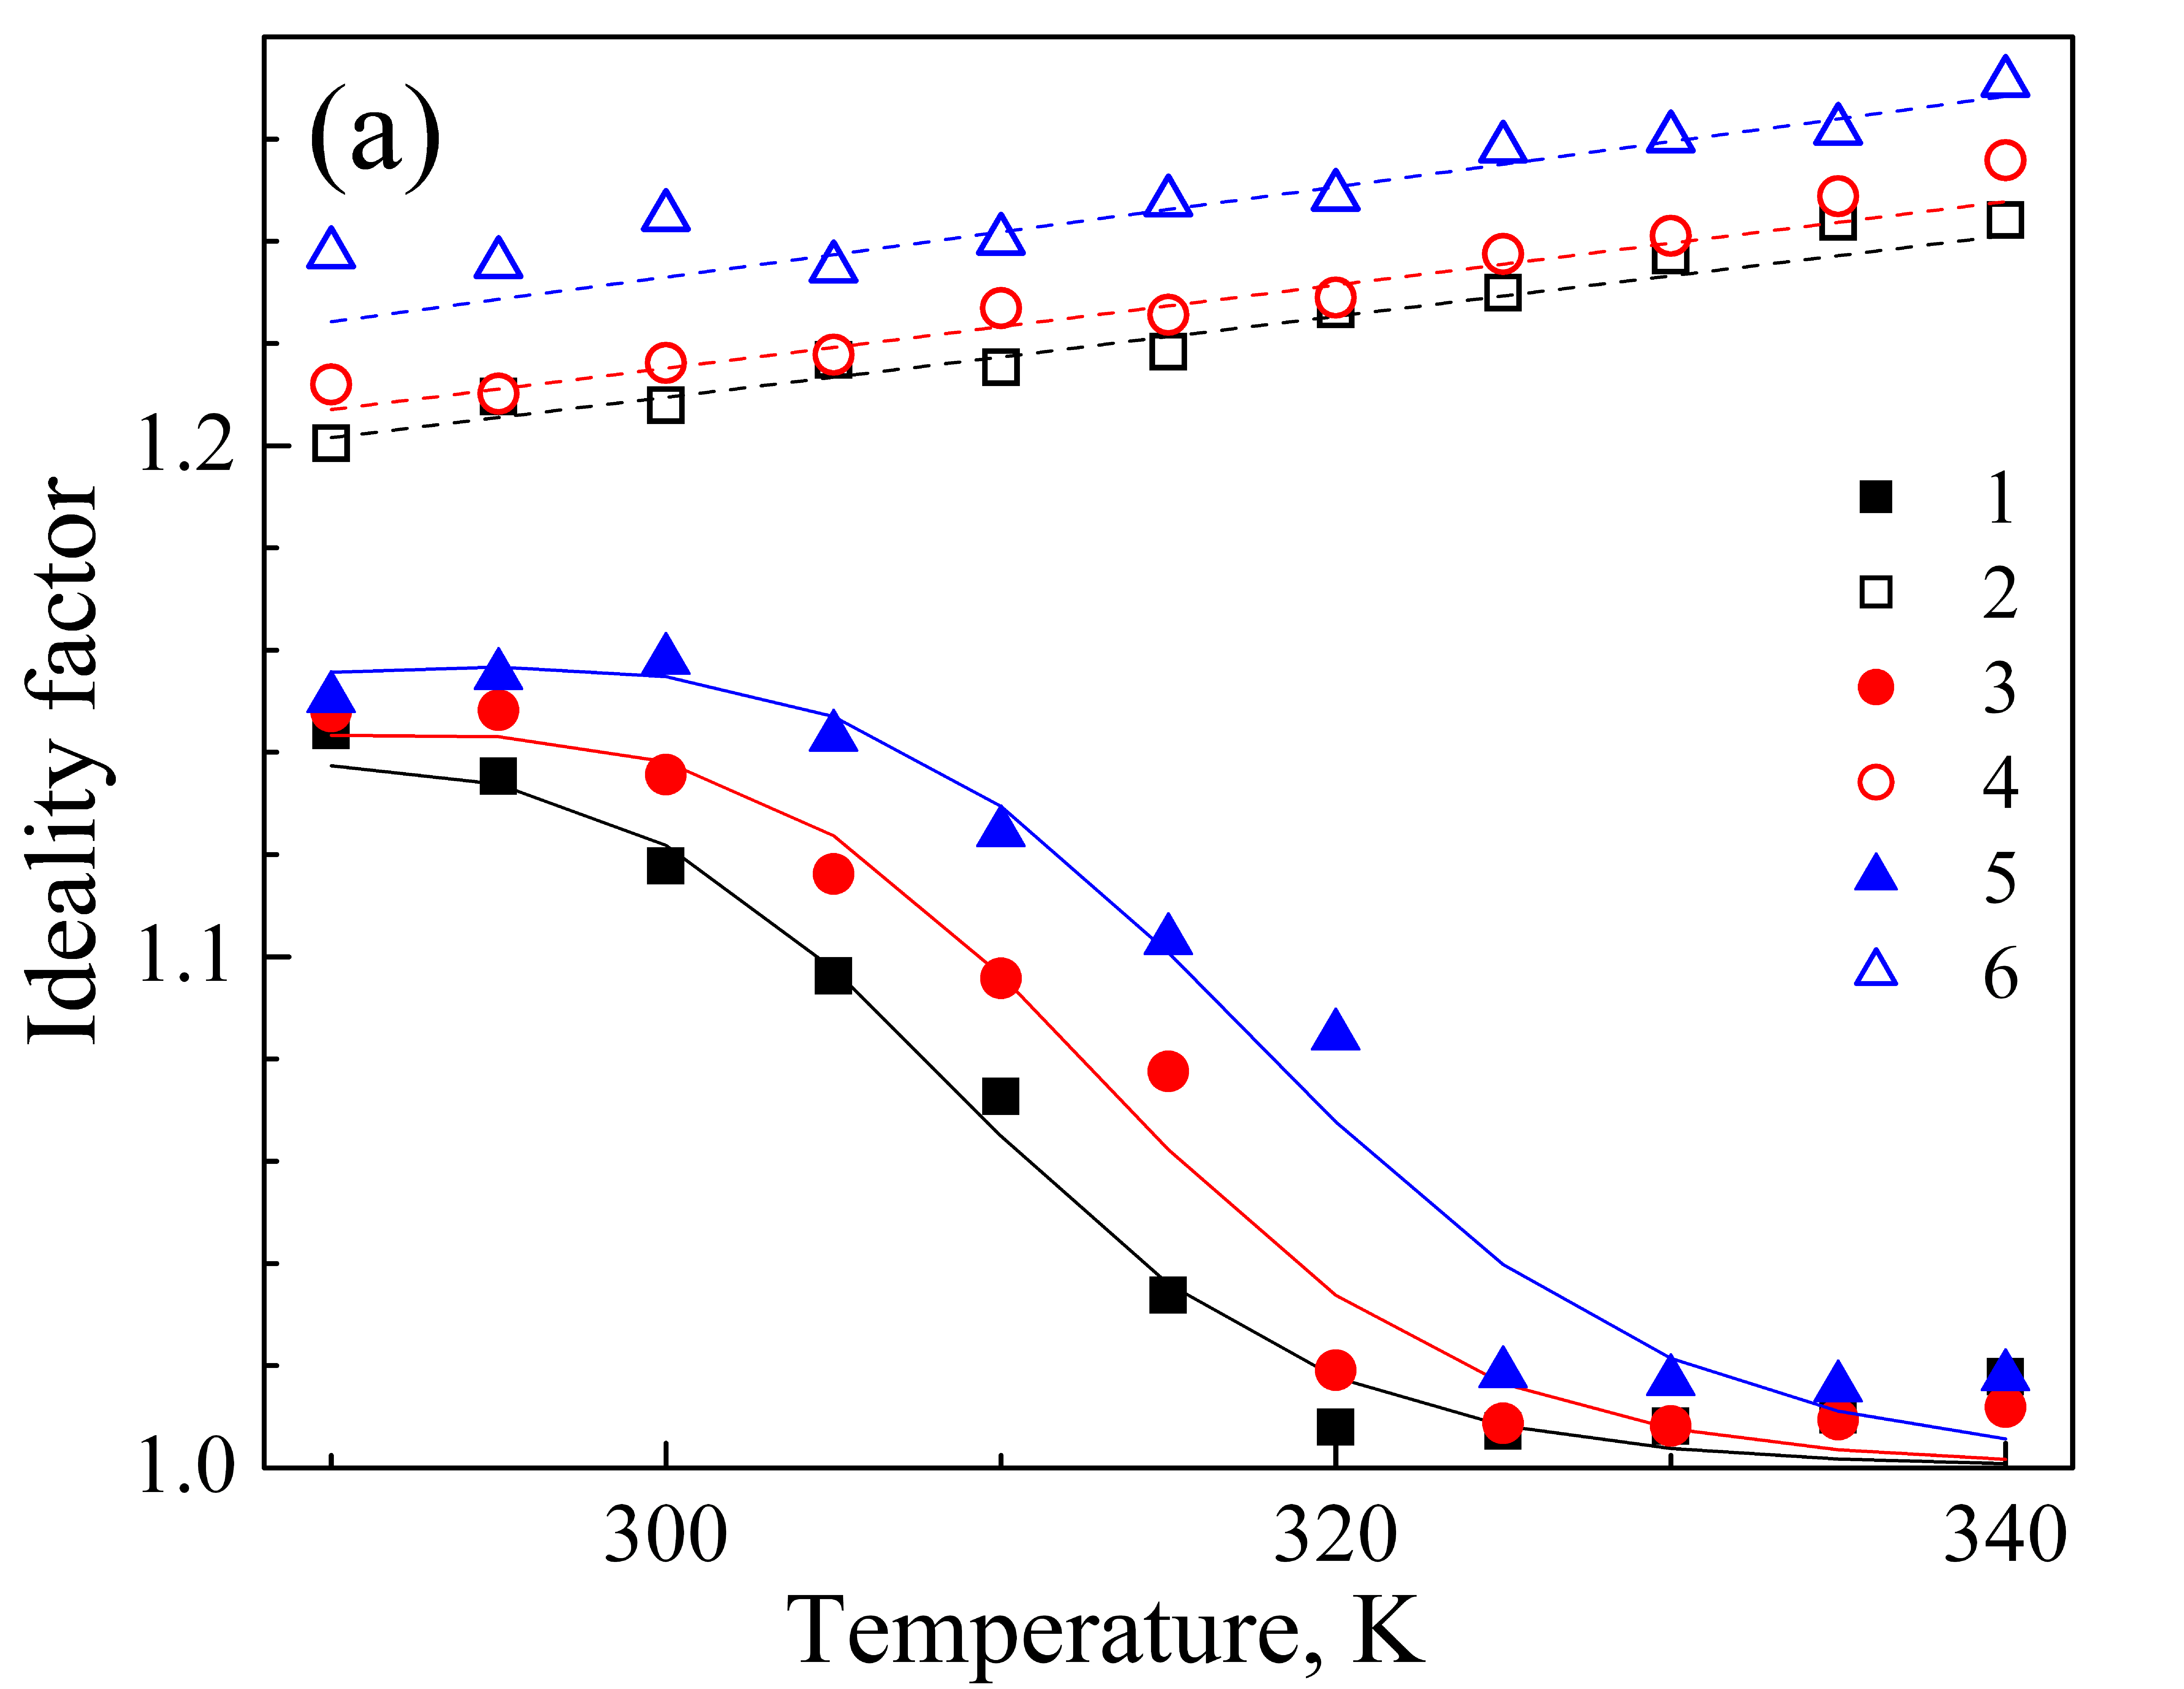
\includegraphics[width=0.5\textwidth]{FigS4a}%

\includegraphics[width=0.5\textwidth]{FigS4b}
\caption{\label{figS4}
Ideality factor as a function of the temperature (a), and dopant (boron) concentration (b).
FI--SRH case.
The marks are the simulation results, and the lines are the fitted curves using Eq.~(5) and data in Table~1.
$N_\mathrm{Fe}$, cm$^{-3}$: $10^{10}$ (curves 1, 2, 7, 8, and 9), $10^{12}$ (3, 4), $10^{13}$ (5, 6, 10, 11, and 12).
$N_\mathrm{A}$ cm$^{-3}$: $10^{15}$ (1, 3, and 5), $10^{17}$ (2, 4, and 6).
$T$, K: 290 (8, 11), 315 (7, 10), 340 (9, 12).
}%
\end{figure}

\begin{figure}
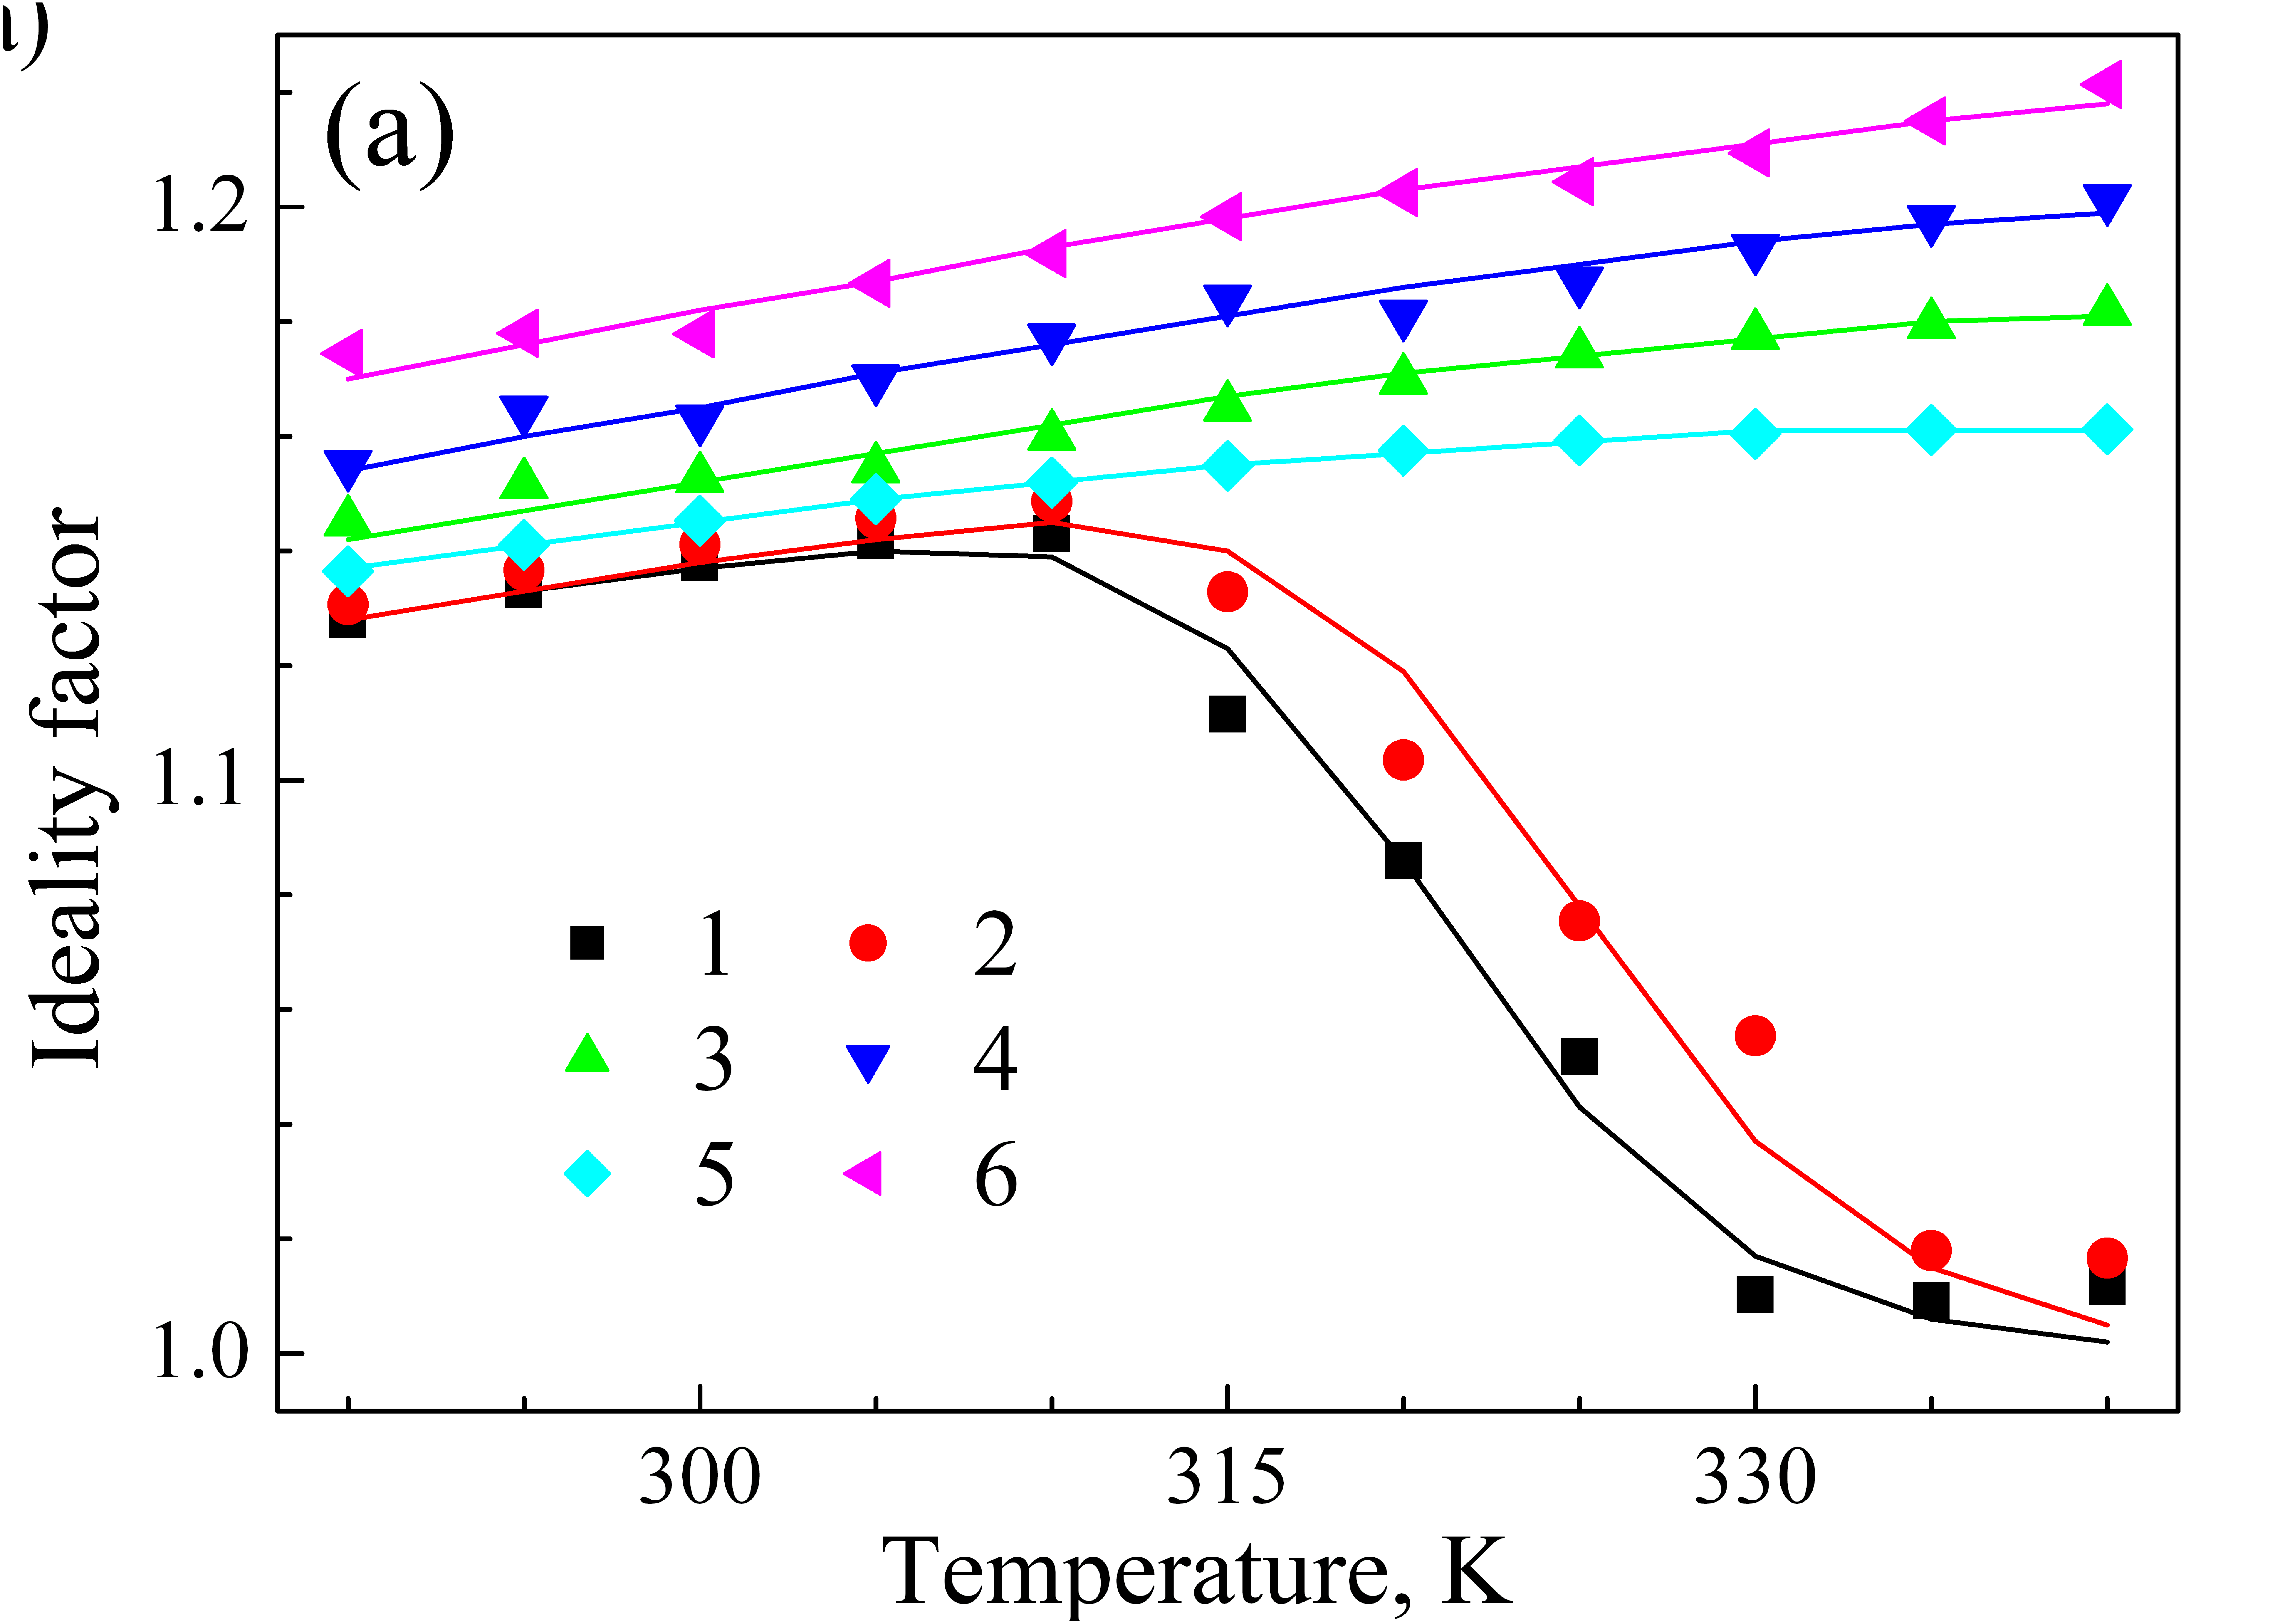
\includegraphics[width=0.5\textwidth]{FigS6a}%
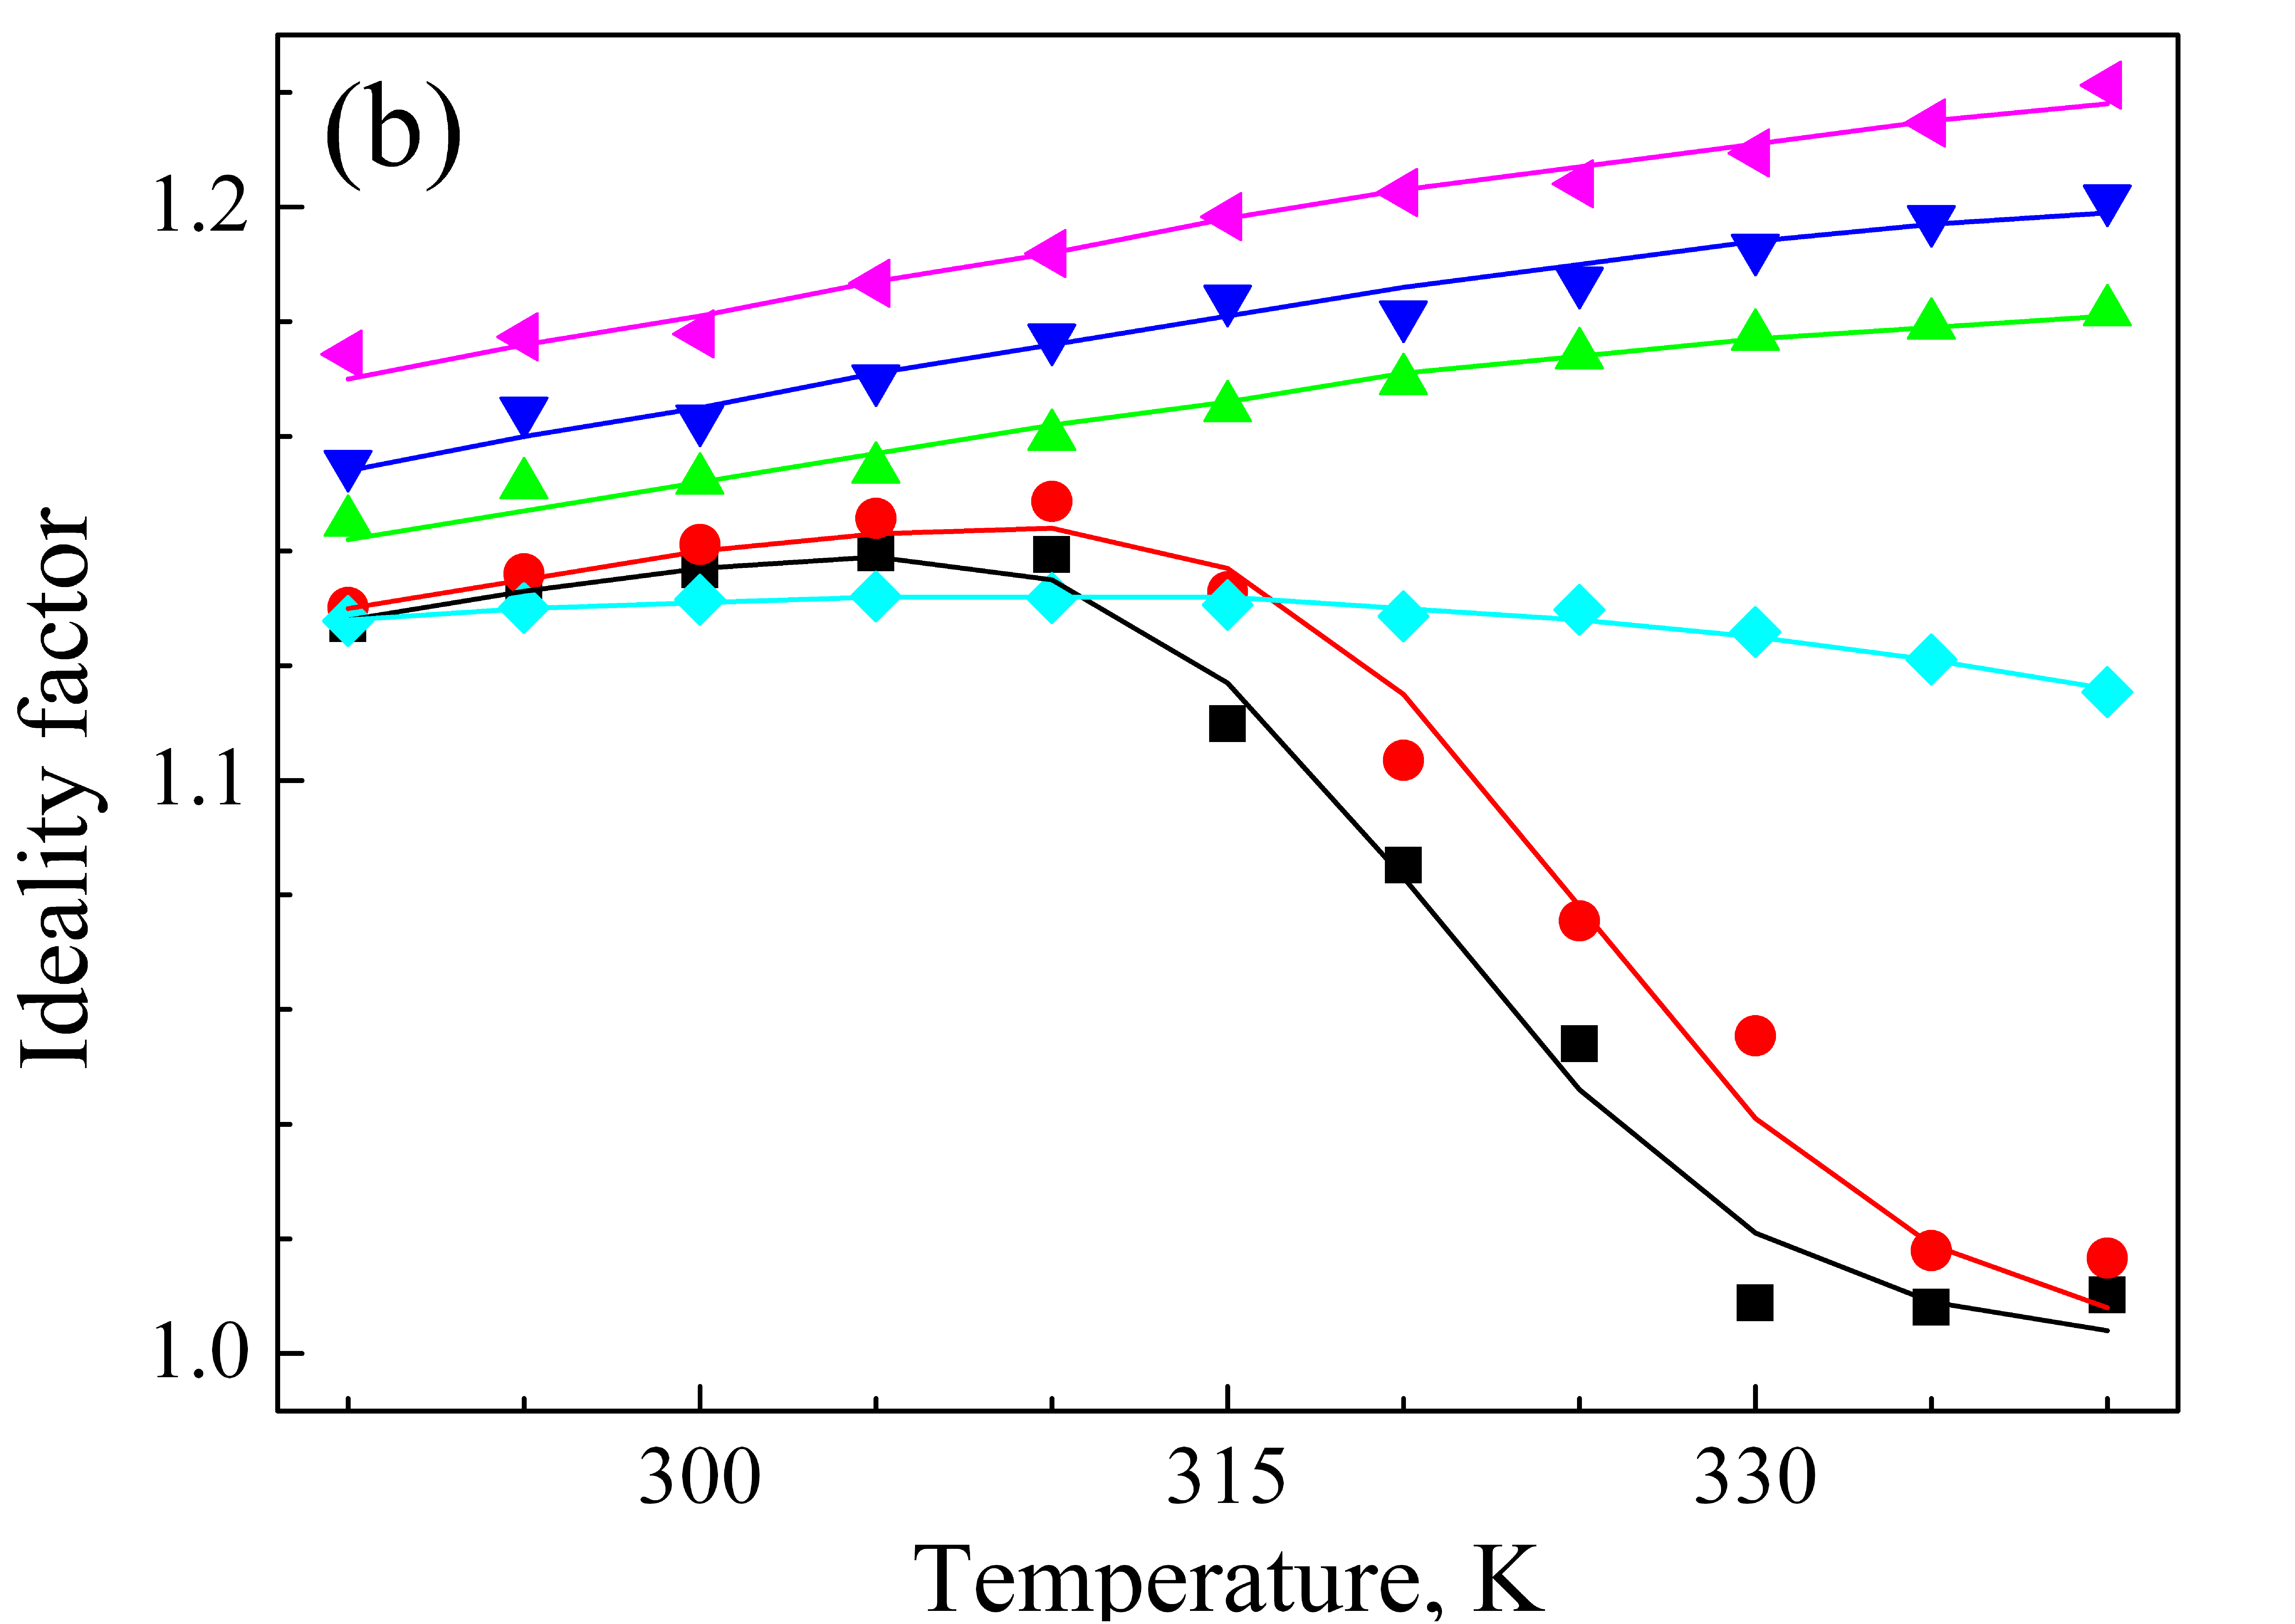
\includegraphics[width=0.5\textwidth]{FigS6b}
\caption{\label{figS6}
Temperature dependencies of the ideality factor.
FIFB--SRH (a) and FIFB--SRHBBA (b) cases.
The marks are the simulation results, and the lines are the fitted curves using Eq.~(5) and data in Table~1.
$N_\mathrm{Fe}$, cm$^{-3}$: $10^{10}$ (curves 1, 5), $10^{12}$ (3), $10^{13}$ (2, 4, and 6).
$N_\mathrm{A}$ cm$^{-3}$: $10^{15}$ (1, 2), $10^{16}$ (3,  4), $10^{17}$ (5, 6).
}%
\end{figure}

\end{document}

